\section{\large \textcolor{blue}{As equações de Maxwell}}

\begin{flushleft}
\textbf{\textcolor{blue}{\Large Quest\~ao 38}}\\
\noindent

\subsection{Quest\~ao 38 IFSP 2015 - Solenoide}
Um campo magn\'etico uniforme faz um \^angulo de $30^\circ$ com o eixo de um enrolamento circular de 
300 voltas e raio de 4 cm. O m\'odulo do campo magn\'etico aumenta a uma taxa de $85\ \text{T/s}$, enquanto 
sua dire\c{c}\~ao permanece fixa. Encontre o m\'odulo da for\c{c}a eletromotriz induzida no enrolamento. 


\begin{itemize}
\item[(A)] 64 V
\item[(B)] 51 V
\item[(C)] 111 V
\item[(D)] 127 V
\item[(E)] 220 V
\end{itemize}

\vspace{0.5cm}

\textcolor{red}{\textbf{Solução:}}\\

Utilizamos a Lei de Faraday da indu\c{c}\~ao eletromagn\'etica:

\[
\mathcal{E} = N \cdot \left| \frac{d\Phi_B}{dt} \right|
\]

O fluxo magn\'etico em uma espira \'e dado por:

\[
\Phi_B = B \cdot A \cdot \cos\theta
\]

Como a dire\c{c}\~ao e a \'area permanecem constantes, temos:

\[
\frac{d\Phi_B}{dt} = A \cdot \cos\theta \cdot \frac{dB}{dt}
\]

Substituindo na express\~ao da f.e.m.:

\[
\mathcal{E} = N \cdot A \cdot \cos\theta \cdot \frac{dB}{dt}
\]

\textbf{Dados:}
\begin{itemize}
    \item $N = 300$
    \item $r = 4\ \text{cm} = 0{,}04\ \text{m} \Rightarrow A = \pi r^2 = \pi \cdot (0{,}04)^2 = 5{,}0265 \times 10^{-3}\ \text{m}^2$
    \item $\frac{dB}{dt} = 85\ \text{T/s}$
    \item $\cos(30^\circ) = 0{,}87$
\end{itemize}

Substituindo:

\[
\mathcal{E} = 300 \cdot (5{,}0265 \times 10^{-3}) \cdot 0{,}87 \cdot 85
\]

\[
\mathcal{E} \approx 1{,}3118 \cdot 85 \approx 111{,}5\ \text{V}
\]


A resposta correta é alternativa \colorbox{green!50}{\textbf{C}}.
\end{flushleft}

\noindent\rule{\linewidth}{0.6pt}\\

\begin{flushleft}
\textbf{\textcolor{blue}{\Large Quest\~ao 39 - IFSP 2015}}\\
\noindent

\subsection{Quest\~ao 39 - IFSP 2015 - Corrente de deslocamento de Maxwell}
Um capacitor de placas paralelas tem placas circulares de raio $R$ com pequena distância entre elas. 
A carga está fluindo a uma taxa de $3{,}0 \ \mathrm{C/s}$. Calcule a corrente de deslocamento de Maxwell através 
da superfície $S$ entre as placas.

\begin{figure}[!h]
\centering
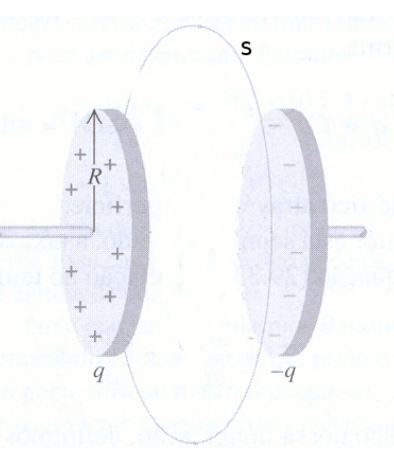
\includegraphics[scale=0.5]{figures/capacitor.png}
\end{figure}    

\begin{itemize}
\item[(A)] Zero
\item[(B)] 1,0 A
\item[(C)] 1,5 A
\item[(D)] 3,0 A
\item[(E)] 4,5 A
\end{itemize}

\vspace{0.5cm}

\textcolor{red}{\textbf{Solução:}}\\

A corrente de deslocamento de Maxwell é dada por: 

\[
i_d = \varepsilon_0 \frac{d\Phi_E}{dt}
\]

onde:
\begin{itemize}
  \item $i_d$ é a corrente de deslocamento,
  \item $\varepsilon_0$ é a permissividade elétrica do vácuo,
  \item $\Phi_E$ é o fluxo elétrico através da superfície $S$ entre as placas do capacitor.
\end{itemize}

O fluxo elétrico é definido como:

\[
\Phi_E = E \cdot A
\]

Sabemos que entre as placas de um capacitor o campo elétrico é:

\[
E = \frac{\sigma}{\varepsilon_0} = \frac{q}{\varepsilon_0 A}
\]

Logo, o fluxo elétrico será:

\[
\Phi_E = \frac{q}{\varepsilon_0}
\]

Substituindo na equação da corrente de deslocamento:

\[
i_d = \varepsilon_0 \cdot \frac{d}{dt} \left( \frac{q}{\varepsilon_0} \right) = \frac{dq}{dt}
\]

Ou seja, a corrente de deslocamento é numericamente igual à taxa de variação da carga no capacitor. Como a taxa de variação da carga é:

\[
\frac{dq}{dt} = 3{,}0 \ \mathrm{C/s}
\]

Concluímos que:

\[
\boxed{i_d = 3{,}0 \ \mathrm{A}}
\]

A resposta correta é alternativa \colorbox{green!50}{\textbf{D}}.
\end{flushleft}

\noindent\rule{\linewidth}{0.6pt}\\

\begin{flushleft}
\textbf{\textcolor{blue}{\Large Quest\~ao 35 - IFSP 2017 - Carga no capacitor}}\\
\noindent

\subsection{Quest\~ao 35 - IFSP 2017 - Carga no capacitor}
Dado o circuito composto por uma fonte de tens\~ao $V_0$, um resistor $R$, um capacitor $C$ e uma chave $S$, 
conforme apresentado abaixo. Qual express\~ao apresenta a quantidade de carga em fun\c{c}\~ao do tempo ap\'os 
a chave $S$ fechar o circuito?

\begin{center}
\begin{circuitikz}
\draw
  (0,0) to[battery, l_=$V_0$] (0,2)
  to[switch, l=$S$] (2,2)
  to[R=$R$] (4,2)
  to[C=$C$] (4,0)
  -- (0,0);
\end{circuitikz}
\end{center}

\begin{itemize}
\item[(A)] $q(t) = CV_0 \left[1 - e^{\frac{-t}{RC}}\right]$
\item[(B)] $q(t) = CV_0 \left[1 - e^{\frac{+t}{RC}}\right]$
\item[(C)] $q(t) = CV_0 \left[1 + e^{\frac{t}{RC}}\right]$
\item[(D)] $q(t) = CV_0 \left[1 + e^{\frac{+t}{RC}}\right]$
\end{itemize}

\vspace{0.5cm}

\textcolor{red}{\textbf{Solução:}}\\

Ao fechar a chave $S$ no instante $t = 0$, a corrente começa a circular no circuito RC s\'erie, carregando o capacitor. A equa\c{c}\~ao que descreve o circuito segundo a Lei de Kirchhoff das malhas é:

\[
V_0 - Ri(t) - \frac{q(t)}{C} = 0
\]

Sabendo que a corrente é a derivada da carga:

\[
i(t) = \frac{dq(t)}{dt}
\]

Substituindo:

\[
V_0 - R \frac{dq(t)}{dt} - \frac{q(t)}{C} = 0
\Rightarrow R \frac{dq(t)}{dt} + \frac{q(t)}{C} = V_0
\]

Essa é uma equa\c{c}\~ao diferencial linear de primeira ordem.

Multiplicando ambos os lados por \( C \):

\[
RC \frac{dq(t)}{dt} + q(t) = CV_0
\]

---

\textbf{Resolvendo a equação diferencial:}

Essa é uma equação linear do tipo:

\[
\frac{dq}{dt} + \frac{1}{RC} q = \frac{V_0}{R}
\]

Usamos o fator integrante \( \mu(t) = e^{t/RC} \):

\[
\frac{d}{dt} \left( q(t) \cdot e^{t/RC} \right) = \frac{V_0}{R} e^{t/RC}
\]

Integrando ambos os lados:

\[
q(t) \cdot e^{t/RC} = \int \frac{V_0}{R} e^{t/RC} dt = \frac{V_0}{R} \cdot RC \cdot e^{t/RC} + C_1
\]

\[
q(t) \cdot e^{t/RC} = CV_0 \cdot e^{t/RC} + C_1
\Rightarrow q(t) = CV_0 + C_1 \cdot e^{-t/RC}
\]

Usando a condi\c{c}\~ao inicial: \( q(0) = 0 \)

\[
0 = CV_0 + C_1 \Rightarrow C_1 = -CV_0
\]

Logo:

\[
q(t) = CV_0 \left(1 - e^{-t/RC} \right)
\]

---

\textbf{Conclus\~ao:}

A carga no capacitor em fun\c{c}\~ao do tempo \'e:

\[
\boxed{q(t) = CV_0 \left(1 - e^{-t/RC} \right)}
\]

Essa expressão mostra que a carga cresce exponencialmente com o tempo até atingir o valor máximo \( CV_0 \), com constante de tempo \( \tau = RC \).

A resposta correta é alternativa \colorbox{green!50}{\textbf{A}}.
\end{flushleft}


\noindent\rule{\linewidth}{0.6pt}\\

\begin{flushleft}
\textbf{\textcolor{blue}{\Large Quest\~ao 49}}\\
\noindent
\subsection{Quest\~ao 49 - Campo elétrico induzido por uma onda eletromagnética}
Considere uma região no espaço onde existe um campo elétrico variável no tempo, dado por $\vec{E} = E_0 \sin(\omega t) \, \hat{z},$
sendo \(E_0\) a amplitude do campo elétrico, \(\omega\) a frequência angular e \(t\) o tempo. De acordo com as equações de Maxwell, 
esse campo elétrico variável irá induzir um campo magnético também variável, dando origem a uma onda eletromagnética. Supondo que a 
onda eletromagnética se propague na direção \(+y\) e que não haja cargas livres ou correntes na região, a expressão que descreve o 
campo magnético \(B\) induzido nessa região é:


\begin{itemize}
\item[(A)] $B = \frac{ E_0}{c} \sin(\omega t) \, \hat{x}.$
\item[(B)] $B = -\frac{E_0}{c} \sin(\omega t) \, \hat{x}.$
\item[(C)] $B = \frac{E_0}{c} \cos(\omega t) \, \hat{x}.$
\item[(D)] $B = -\frac{E_0}{c} \cos(\omega t) \, \hat{x}.$
\end{itemize}

\vspace{0.5cm}

\textcolor{red}{\textbf{Solução:}}\\



\section*{1. Forma geral da onda eletromagnética no vácuo}

No vácuo, uma onda plana que se propaga na direção \(+\hat{y}\) tem os campos elétrico e magnético na forma:
\[
\vec{E}(y,t) = E_0 \sin(k y - \omega t) \, \hat{z},
\]
\[
\vec{B}(y,t) = B_0 \sin(k y - \omega t) \, \hat{x}.
\]

A relação entre as amplitudes \(E_0\) e \(B_0\) é dada por:
\[
B_0 = \frac{E_0}{c}.
\]

Considere a região do espaço onde o campo elétrico é dado por:
\[
\vec{E}(y,t) = E_0 \sin(k y - \omega t) \, \hat{z}.
\]

Queremos determinar o campo magnético associado \(\vec{B}(y,t)\), calculando o rotacional de \(\vec{E}\) e usando a \textbf{lei de Faraday}:
\[
\nabla \times \vec{E} = -\frac{\partial \vec{B}}{\partial t}.
\]

\section*{2. Cálculo do rotacional de \(\vec{E}\)}

O campo elétrico tem apenas a componente \(z\), que depende apenas de \(y\) e \(t\).  
Em coordenadas cartesianas:
\[
\nabla \times \vec{E} =
\begin{vmatrix}
\hat{x} & \hat{y} & \hat{z} \\[4pt]
\partial_x & \partial_y & \partial_z \\[4pt]
0 & 0 & E_z
\end{vmatrix}
=
\left( \frac{\partial E_z}{\partial y} \right) \hat{x} - \left( \frac{\partial E_z}{\partial x} \right) \hat{y} + 0 \, \hat{z}.
\]

Como \(E_z = E_0 \sin(k y - \omega t)\), temos:
\[
\frac{\partial E_z}{\partial y} = k E_0 \cos(k y - \omega t),
\quad
\frac{\partial E_z}{\partial x} = 0.
\]

Assim:
\[
\nabla \times \vec{E} = k E_0 \cos(k y - \omega t) \, \hat{x}.
\]

\section*{3. Lei de Faraday}

Pela lei de Faraday:
\[
\nabla \times \vec{E} = -\frac{\partial \vec{B}}{\partial t}.
\]

Logo:
\[
\frac{\partial \vec{B}}{\partial t} = -\nabla \times \vec{E} = -k E_0 \cos(k y - \omega t) \, \hat{x}.
\]

\section*{4. Integração no tempo}

Para encontrar \(\vec{B}(y,t)\), integramos no tempo:
\[
\vec{B}(y,t) = \int \frac{\partial \vec{B}}{\partial t} \, dt = -k E_0 \int \cos(k y - \omega t) \, dt \, \hat{x}.
\]

Como \(y\) é constante na derivada temporal, podemos integrar diretamente:
\[
\int \cos(k y - \omega t) \, dt = -\frac{1}{\omega} \sin(k y - \omega t).
\]

Portanto:
\[
\vec{B}(y,t) = \frac{k E_0}{\omega} \sin(k y - \omega t) \, \hat{x}.
\]

\section*{5. Relação entre \(k\), \(\omega\) e \(c\)}

No vácuo, sabemos que:
\[
c = \frac{\omega}{k} \quad \text{ou equivalentemente} \quad \frac{k}{\omega} = \frac{1}{c}.
\]

Substituindo:
\[
\vec{B}(y,t) = \frac{E_0}{c} \sin(k y - \omega t) \, \hat{x}.
\]

\section*{6. Resposta final}

Portanto, a expressão para o campo magnético induzido é:
\[
\boxed{
\vec{B}(y,t) = \frac{E_0}{c} \sin(k y - \omega t) \, \hat{x}
}
\]


A resposta correta é alternativa \colorbox{green!50}{\textbf{A}}.
\end{flushleft}

\noindent\rule{\linewidth}{0.6pt}\\

\begin{flushleft}
\textbf{\textcolor{blue}{\Large Quest\~ao 50}}\\
\noindent
\subsection{Quest\~ao 50 - Lei de Gauss para dielétricos homogêneos}
Considere uma esfera de raio \( R \) feita de um material dielétrico linear e homogêneo com permissividade elétrica \( \varepsilon \).  
Uma carga total \( +Q \) está uniformemente distribuída no volume da esfera. De acordo com a lei de Gauss, o campo elétrico \( E \) 
dentro (\( r < R \)) e fora (\( r \geq R \)) da esfera é:


\begin{itemize}
\item[(A)] $\frac{Q}{4\pi\varepsilon R^3} \, \hat{\textrm{r}} \quad \text{se} \quad r < R \quad e \quad \frac{Q}{4\pi\varepsilon_0 r^2} \, \hat{\textrm{r}} \quad \text{se} \quad r \geq R. $
\item[(B)] $\frac{Q r^2}{4\pi\varepsilon R^2} \, \hat{\textrm{r}} \quad \text{se} \quad r < R \quad e \quad \frac{Q}{4\pi\varepsilon_0 r^2} \, \hat{\textrm{r}}  \quad \text{se} \quad r \geq R.$
\item[(C)] $\frac{Q r}{4\pi\varepsilon R^3} \, \hat{\textrm{r}} \quad \text{se} \quad r < R \quad e \quad \frac{Q}{4\pi\varepsilon_0 r^2} \, \hat{\textrm{r}} \quad \text{se} \quad r \geq R.$
\item[(D)] $\frac{Q r}{4\pi\varepsilon R^2} \, \hat{\textrm{r}} \quad \text{se} \quad r < R \quad e \quad \frac{Q}{4\pi\varepsilon_0 r^2} \, \hat{\textrm{r}} \quad \text{se} \quad r \geq R.$
\end{itemize}

\vspace{0.5cm}

\begin{center}
\textbf{Superfícies gaussianas para os casos \(r<R\) e \(r\geq R\)}
\end{center}

\begin{center}
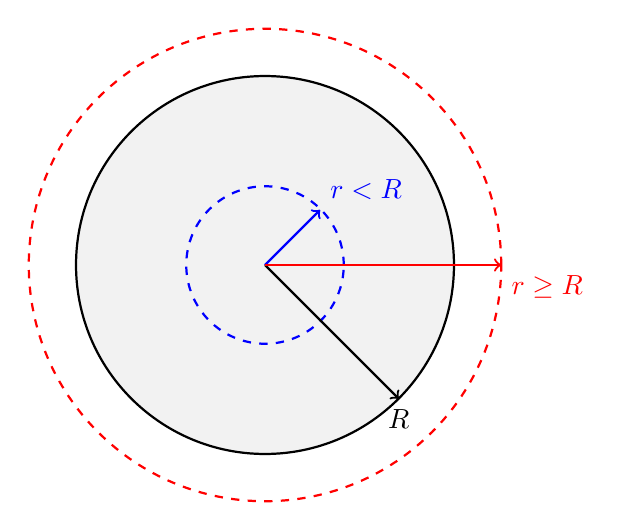
\begin{tikzpicture}[scale=2]

% Esfera carregada
\fill[gray!10] (0,0) circle (1.2);
\draw[thick] (0,0) circle (1.2);
%\node at (0,0) {\( +Q \) uniformemente distribuído};

% Superfície gaussiana interna (r<R)
\draw[dashed, blue, thick] (0,0) circle (0.5);
%\node[blue] at (0.75,0.2) {\( r<R \)};

% Superfície gaussiana externa (r>R)
\draw[dashed, red, thick] (0,0) circle (1.5);
%\node[red] at (1.7,0.2) {\( r\geq R \)};

% Marcas de raio R
\draw[thick,->] (0,0) -- (0.85,-0.85) node[below] {\(R\)};

% Raio interno
\draw[thick,->,blue] (0,0) -- (0.35,0.35) node[above right] {\(r<R\)};

% Raio externo
\draw[thick,->,red] (0,0) -- (1.5,0) node[below right] {\(r\geq R\)};

\end{tikzpicture}
\end{center}

\textcolor{red}{\textbf{Solução:}}\\

\section*{1. Densidade de carga volumétrica}

A carga está uniformemente distribuída no volume da esfera:
\[
\rho = \frac{Q}{\frac{4}{3} \pi R^3} = \frac{3Q}{4\pi R^3}.
\]

\section*{2. Lei de Gauss para dielétricos}

No material dielétrico, o campo elétrico \( \vec{E} \) está relacionado ao deslocamento elétrico \( \vec{D} \) por:
\[
\vec{D} = \varepsilon \vec{E}.
\]

A lei de Gauss para \( \vec{D} \) em forma integral:
\[
\oint_{S} \vec{D} \cdot d\vec{A} = Q_{\text{int}}.
\]

Para simetria esférica, escolhemos uma superfície gaussiana esférica de raio \( r \).  

---

\section*{3. Campo dentro da esfera (\( r < R \))}

A carga contida em uma esfera de raio \( r < R \) é:
\[
Q_{\text{int}}(r) = \rho \cdot \frac{4}{3} \pi r^3.
\]

Aplicando a lei de Gauss para \( D_r \):
\[
D_r \cdot 4\pi r^2 = Q_{\text{int}}(r) \quad \Rightarrow \quad D_r = \frac{\rho r}{3}.
\]

Como \( \vec{E} = \vec{D}/\varepsilon \), temos:
\[
E_r(r<R) = \frac{D_r}{\varepsilon} = \frac{\rho r}{3\varepsilon}.
\]

Substituindo \(\rho\):
\[
E_r(r<R) =
\frac{1}{3\varepsilon} \cdot \frac{3Q}{4\pi R^3} \cdot r =
\frac{Q r}{4\pi \varepsilon R^3}.
\]

---

\section*{4. Campo fora da esfera (\( r \geq R \))}

Para \( r \geq R \), toda a carga \( Q \) está contida:
\[
D_r \cdot 4\pi r^2 = Q \quad \Rightarrow \quad D_r = \frac{Q}{4\pi r^2}.
\]

Logo:
\[
E_r(r \geq R) =
\frac{D_r}{\varepsilon} =
\frac{Q}{4\pi \varepsilon r^2}.
\]

---

\section*{5. Resposta final}

O campo elétrico \( E_r \) em todos os pontos do espaço é dado por:
\[
\boxed{
E_r(r) =
\begin{cases}
\dfrac{Q r}{4\pi \varepsilon R^3}, & r < R \\[12pt]
\dfrac{Q}{4\pi \varepsilon r^2}, & r \geq R
\end{cases}
}
\]

A resposta correta é alternativa \colorbox{green!50}{\textbf{C}}.
\end{flushleft}

\begin{center}
\textbf{Campo elétrico \(E(r)\) em função de \(r\)}
\end{center}

O campo elétrico radial \(E(r)\) em uma esfera uniformemente carregada com raio \(R\) é dado por:
\[
E(r) =
\begin{cases}
\displaystyle \frac{Q r}{4\pi \varepsilon R^3}, & r < R \\[12pt]
\displaystyle \frac{Q}{4\pi \varepsilon r^2}, & r \geq R
\end{cases}
\]

O gráfico abaixo mostra qualitativamente o comportamento de \(E(r)\) em função de \(r\).

\bigskip

\begin{center}
\begin{tikzpicture}
\begin{axis}[
    axis lines = left,
    xlabel = {$r$},
    ylabel = {$E(r)$},
    xmin=0, xmax=2,
    ymin=0, ymax=1.2,
    xtick={0.5,1,1.5},
    xticklabels={$0.5R$,$R$,$1.5R$},
    ytick=\empty,
    domain=0:2,
    samples=100,
    width=12cm,
    height=8cm
]

% Dentro da esfera: E ~ r
\addplot[blue, thick, domain=0:1] {x};
% Fora da esfera: E ~ 1/r^2
\addplot[blue, thick, domain=1:2] {1/(x*x)};

% Linha pontilhada em r=R
\draw[dashed] (axis cs:1,0) -- (axis cs:1,1);

% Marca R no eixo x
\node[below] at (axis cs:1,0) {$R$};

\end{axis}
\end{tikzpicture}
\end{center}

\begin{flushleft}
\textbf{\textcolor{blue}{\Large Quest\~ao 27}}\\
\subsection{Quest\~ao 27 - Lei de Faraday/Lei de Ohm}
Um fio condutor em formato de armação quadrada de lado $50 \ \text{cm}$ está inicialmente em repouso dentro 
de uma região com campo magnético uniforme de $0{,}8 \ \text{T}$, perpendicular ao plano do circuito. Em determinado instante, 
o fio começa a ser puxado para fora da região do campo magnético com velocidade constante de $5 \ \text{m/s}$, de modo que a 
extremidade do quadrado atravessa a borda do campo magnético. Sabendo que o fio possui resistência elétrica de $10^{-3} \ \Omega/\text{cm}$, 
qual é a corrente elétrica induzida no circuito durante o movimento?


\begin{itemize}
\item[(A)] 3{,}0 A.
\item[(B)] 4{,}8 A.  
\item[(C)] 6{,}0 A.
\item[(D)] 8{,}2 A.
\item[(E)] 10{,}0 A.
\end{itemize}

\vspace{0.5cm}

\textcolor{red}{\textbf{Solução:}}\\

\begin{itemize}
    \item Lado do quadrado: $L = 0,5 \ \text{m}$
    \item Campo magnético: $B = 0,8 \ \text{T}$
    \item Velocidade com que a armação é puxada: $v = 5 \ \text{m/s}$
    \item Resistência linear do fio: $r = 10^{-3} \ \Omega/\text{cm} = 0,1 \ \Omega/\text{m}$
\end{itemize}

\begin{center}
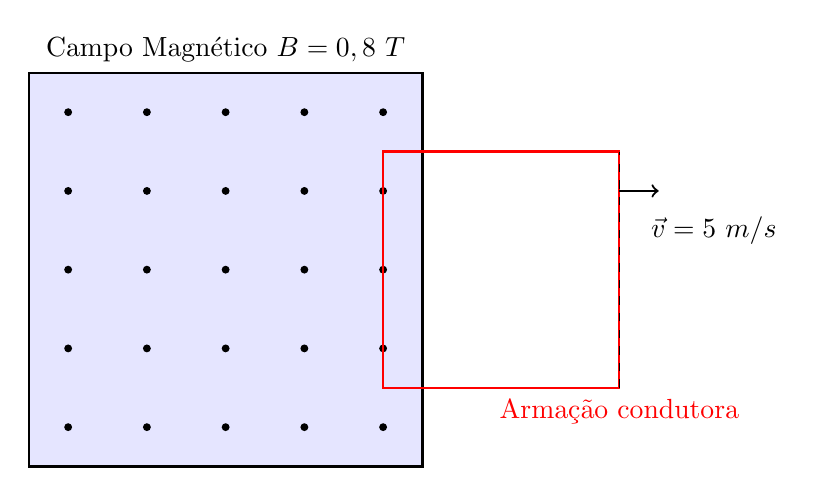
\begin{tikzpicture}

    % Área do campo magnético
    \fill[blue!10] (0,0) rectangle (5,5);
    \draw[thick] (0,0) rectangle (5,5);
    \node at (2.5,5.3) {Campo Magnético $B = 0,8 \ \text{T}$};

    % Indicação das linhas de campo magnético (pontos saindo da folha)
    \foreach \x in {0.5,1.5,2.5,3.5,4.5} {
        \foreach \y in {0.5,1.5,2.5,3.5,4.5} {
            \fill[black] (\x,\y) circle (0.05);
        }
    }
    %\node at (5.5,2.5) {Borda do campo};

    % Armação quadrada
    \draw[red, thick] (4.5,1) -- (4.5,4) -- (7.5,4) -- (7.5,1) -- cycle;
    \node[red] at (7.5,0.7) {Armação condutora};

    % Vetor velocidade
    \draw[->, thick] (7.5,3.5) -- (8,3.5);
    \node at (8.7,3.0) {$\vec{v} = 5 \ \text{m/s}$};

    % Indicação da direção de movimento da armação
    \draw[dashed] (7.5,1) -- (7.5,4);

\end{tikzpicture}
\end{center}

\textbf{1) Força eletromotriz induzida (fem):}

Durante o movimento, a variação do fluxo magnético induz uma força eletromotriz.

A \textbf{fem induzida} pode ser calculada pela expressão:

\[
\boxed{
\mathcal{E} = -\frac{d\Phi}{dt}} \quad \text{Lei de Faraday
}
\]

\[
\mathcal{E} = B \cdot L \cdot \frac{dx}{dt}
\]

\[
\mathcal{E} = B \cdot L \cdot v
\]

Onde:

\begin{itemize}
    \item $L$ é o comprimento da parte do fio que atravessa o campo (no caso, o lado da armação, pois a borda avançando corta uma área de largura $L$).
\end{itemize}

Substituindo:

\[
\mathcal{E} = 0,8 \cdot 0,5 \cdot 5 = 2,0 \ \text{V}
\]

\textbf{2) Resistência total do circuito:}

O comprimento total do fio é o perímetro da armação quadrada:

\[
\ell = 4 \cdot L = 4 \times 0,5 = 2,0 \ \text{m}
\]

Então, a resistência total $R$ será:

\[
R = r \cdot \ell = 0,1 \cdot 2,0 = 0,2 \ \Omega
\]

\textbf{3) Corrente induzida:}

Pela Lei de Ohm:

\[
I = \frac{\mathcal{E}}{R} = \frac{2,0}{0,2} = 10 \ \text{A}
\]

\textbf{Resposta:}

\[
\boxed{I = 10 \ \text{A}}
\]

\textbf{Resposta correta: \colorbox{green!50}{(E)}}

\end{flushleft}

\begin{flushleft}
\textbf{\textcolor{blue}{\Large Quest\~ao 23 - IFFAR 2023 - Associa\c{c}\~ao de Lentes Delgadas}}\\
\noindent

\subsection*{Quest\~ao 23 - IFFAR 2023 - Associa\c{c}\~ao de Lentes Delgadas}

Sistemas \'opticos compostos por associa\c{c}\~ao de lentes desempenham um papel fundamental no ensino de f\'isica 
no campo da \'optica geom\'etrica. Eles s\~ao utilizados para produzir imagens com caracter\'isticas especiais, assim 
como aquelas obtidas por microsc\'opios compostos ou lunetas astron\^omicas.

Nesse contexto, considere um caso te\'orico em que duas lentes delgadas, sendo elas coaxiais, s\~ao associadas com 
uma dist\^ancia $d = 15\,cm$ entre elas. As lentes t\^em dist\^ancias focais $f_1 = 10\,cm$ e $f_2 = 2\,cm$.

Qual \'e a verg\^encia equivalente da associa\c{c}\~ao das lentes?

\begin{itemize}
\item[(A)] $-0{,}07\,di$
\item[(B)] $-15\,di$
\item[(C)] $0{,}02\,di$
\item[(D)] $12\,di$
\item[(E)] $60\,di$
\end{itemize}

\vspace{0.5cm}

\textcolor{red}{\textbf{Solu\c{c}\~ao:}}\\

Quando duas lentes delgadas s\~ao associadas a uma certa dist\^ancia $d$ entre si, a verg\^encia equivalente do sistema \'optico \'{e} dada por:

\[
V = V_1 + V_2 - d \cdot V_1 \cdot V_2
\]

Onde:
\begin{itemize}
    \item $V_1 = \dfrac{100}{f_1}$, com $f_1$ em cm
    \item $V_2 = \dfrac{100}{f_2}$, com $f_2$ em cm
    \item $d$ \'e a dist\^ancia entre as lentes, em metros
\end{itemize}

Calculamos as verg\^encias individuais:

\[
V_1 = \frac{100}{10} = 10\,di
\qquad
V_2 = \frac{100}{2} = 50\,di
\]

Convertendo a dist\^ancia $d$ para metros:

\[
d = 15\,cm = 0{,}15\,m
\]

Substituindo na f\'ormula da verg\^encia equivalente:

\[
V = 10 + 50 - 0{,}15 \cdot 10 \cdot 50
\]

\[
V = 60 - 0{,}15 \cdot 500 = 60 - 75 = -15\,di
\]

\vspace{0.3cm}

Portanto, a resposta correta \'e a alternativa \colorbox{green!50}{\textbf{B)}}.

\end{flushleft}


\begin{flushleft}
\textbf{\textcolor{blue}{\Large Q}}\\
\noindent

\subsection{Quest\~ao }

\begin{itemize}
\item[(A)] 
\item[(B)] 
\item[(C)] 
\item[(D)] 
\item[(E)] 
\end{itemize}

\vspace{0.5cm}

\textcolor{red}{\textbf{Solução:}}\\

A resposta correta é alternativa \colorbox{green!50}{\textbf{...}}.
\end{flushleft}
